\documentclass{article}%
\usepackage[T1]{fontenc}%
\usepackage[utf8]{inputenc}%
\usepackage{lmodern}%
\usepackage{textcomp}%
\usepackage{lastpage}%
\usepackage[head=40pt,margin=0.5in,bottom=0.6in]{geometry}%
\usepackage{graphicx}%
%
\title{\textbf{¿Cuál será el próximo capítulo?}}%
\author{ÁLVARO MONTENEGRO FORTIQUE}%
\date{04/03/2019}%
%
\begin{document}%
\normalsize%
\maketitle%
\textbf{URL: }%
http://www.eluniversal.com/el{-}universal/34298/cual{-}sera{-}el{-}proximo{-}capitulo\newline%
%
\textbf{Periodico: }%
EU, %
ID: %
34298, %
Seccion: %
el{-}universal\newline%
%
\textbf{Palabras Claves: }%
NO\_TIENE\newline%
%
\textbf{Derecho: }%
2.1%
, Otros Derechos: %
\newline%
%
\textbf{\textit{Al final del día no veo la manera de que no se llamen a elecciones libres y transparentes, que den todas las garantías a los ciudadanos venezolanos de que su voluntad será respetada}}%
\newline%
\newline%
%
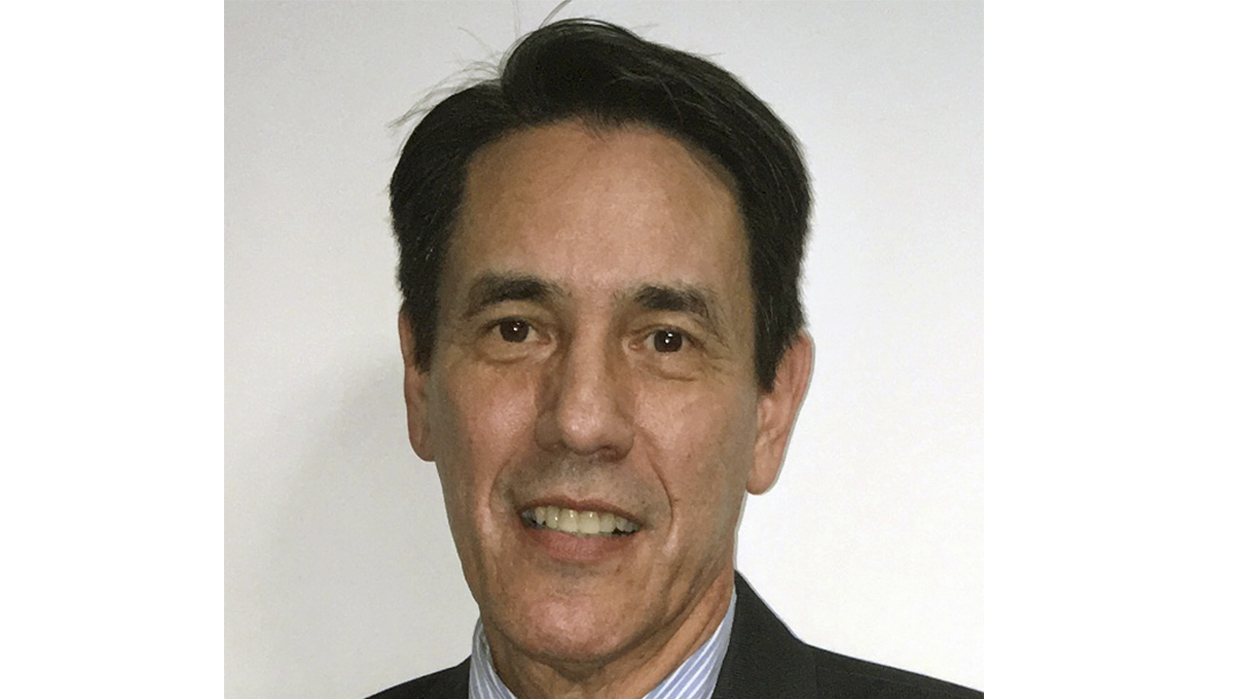
\includegraphics[width=300px]{EU_34298.jpg}%
\newline%
%
Hacer pronósticos en Venezuela en este momento es más difícil que acertar en las  teorías de las ciencias ocultas. Las recetas de magia o los ritos de ocultismo son más fáciles de ejecutar, que adivinar el devenir de nuestro país en el momento que escribo estas líneas. El aspecto que toman los acontecimientos cambia en horas, minutos, y segundos. Las escaladas de “violencia legítima” de Max Weber que han sucedido eran absolutamente imprevistas e innecesarias. Matar indígenas y manifestantes en las fronteras, o quemar camiones que traen comida y medicinas a la población, se convirtieron en muestras de sadismo que no beneficiaron ni a quienes dieron esas órdenes. Al contrario, se transformaron en un motivo privilegiado para aplicar más fogosidad a la situación. Todos sabemos que la violencia siempre trae más violencia. El modo de actuar ante la ayuda humanitaria ha permitido asomar el verdadero rostro de cada quien. Se cayeron las máscaras carnestolendas. Se deshilachan a jirones los disfraces de bondad de algunos, si es que todavía los tenían puestos. El gobierno no ha debido impedir la entrada de ayuda humanitaria, y menos al costo de vidas de ciudadanos indefensos o quemando camiones. Fue muy torpe esa decisión porque perdieron mucho y no ganaron nada.%
\newline%
%
Este carnaval está muy raro. Exageradamente extraño. El humor político del venezolano ha dado un giro en vista a los últimos acontecimientos. La esperanza de un país mejor viene ahora acompañada de una sorda rabia, ocasionada por la estéril y cruel represión. La ansiedad sigue marcando la pauta diaria en la mente de los venezolanos que solo queremos calma, sosiego y serenidad. ¿Cuál será el precio a pagar por obtener esa tranquilidad? ¿Cuántos muertos más, que se convierten a diario en los mártires de esta historia, tendrán que haber para que logremos ser un país normal? Nadie lo sabe. Todos estamos en vilo. En mi último artículo sobre Erasmo de Rotterdam cité su posición frente a los conflictos armados: “La guerra significa necesariamente injusticia, pues generalmente no daña a aquellos que la instigan y la dirigen sino a los inocentes”. No cabe duda de que la factura de las conflagraciones siempre la cancelan los más desamparados.%
\newline%
%
Si bien la forma que toman los acontecimientos sigue tan confusa como una bola de cristal empañada, lo cierto es que el fondo está mucho más claro: Venezuela está cambiando para siempre. Ya nada será como antes. Por más de que la erótica del poder confunda a los dirigentes como la droga engaña al adicto, no hay manera de sostener esta crisis económica y política. Ya son muchos años que tiene el pueblo venezolano sufriendo las consecuencias de malas decisiones públicas. La inflación más alta del mundo en un entorno donde esa enfermedad financiera ya no existe, la pérdida del aparato productivo del país, la escasez de alimentos y medicinas, el insólito deterioro de todos los servicios públicos básicos y la delincuencia incontrolada que se alimenta con una desvergonzada impunidad judicial, han convertido a Venezuela en el nuevo país del éxodo continental. Millones de compatriotas han huido de este desastre. Ya ese conteo, que realizan los organismos especializados de la ONU, asombra hasta al analista más despistado.%
\newline%
%
¿Cuál será el próximo capítulo de esta historia que parece una tragedia griega? Los escenarios son muchos en la forma, pero en el fondo son todos iguales. Esto no lo aguanta nadie, como decía el eslogan de una campaña política del pasado. Al final del día no veo la manera de que no se llamen a elecciones libres y transparentes, que den todas las garantías a los ciudadanos venezolanos de que su voluntad será respetada.%
\newline%
%
alvaromont@gmail.com%
\newline%
%
\end{document}